%%%%%%%%%%%%%%%%%%%%%%%%%%%%%
%Update: <Sep/24/2010>
%%%%%%%%%%%%%%%%%%%%%%%%%%%%%
\chapter{マイクロコンピュータ応用}

\section{目的}

まず, ステッピングモータを理解し, 制御することが今回の目標です。
さらに, スイッチの操作の復習も行います。

\section{装置}

\subsection{ステッピングモータとは}

ステッピングモータは, 普通のモータ異なり, パルス信号が入力されるごとに, 一定の角
度ずつ回転させることができるモータです。一定の角度回転させることができるので, 装
置の位置を制御するのに適しているモータです。

ステッピングモータは周囲に付けられたコイル(ステータ)と, 回転軸に固定された磁石
(ロータ)で構成されます。コイルに電流を流すことで磁界が生じ
(このことを励磁と言います), その磁界により磁石が引き寄せられることで, ステッピン
グモータは一定角度回転します。コイルへの電流の流し方を変
えることで, 異なった性質を持つ回転をつくり出すことができます。


\begin{figure}[htbp]
\begin{center}
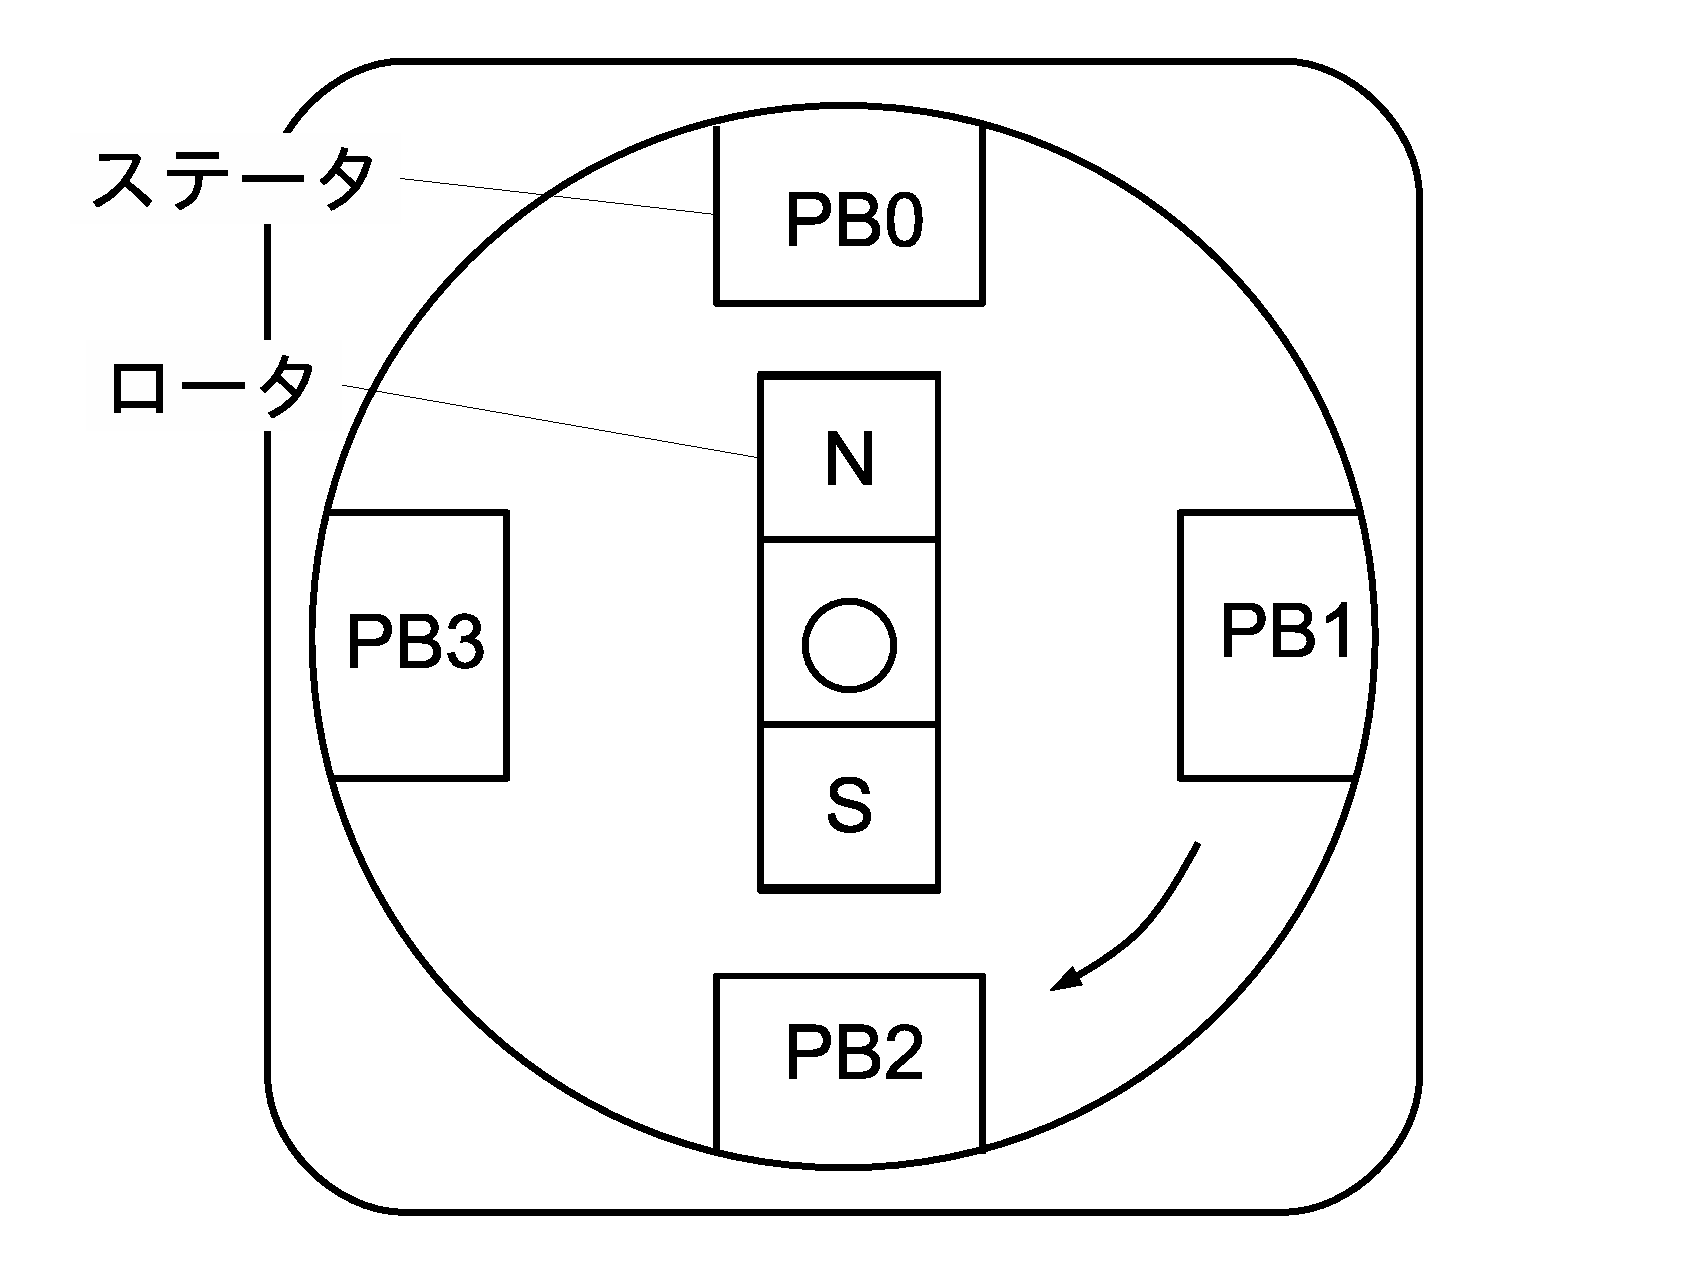
\includegraphics[width=0.5\linewidth]{img/steppingmotor.eps}
\caption{ステッピングモータの概念図。ポートBに電流を流すことで磁界が発生し, 磁石
    が回る。}
\label{fig:steppingmotor}
\end{center}
\end{figure}

\subsection{装置セッティング}

今回はMT-Zの拡張パーツであるステッピングモータを用います。ステッピングモータを使
えるようにするには, まず, ステッピングモータはステッピングモータインターフェース
ボードに接続します。次に, ステッピングモータインターフェースボードにアダプタを接
続します。そして, \figref{fig:connection-motor}のようにステッピングモータインター
フェースボードをMT-Zの左にあるIOポートに繋ぎます。以上のように接続することで, オ
ンボードの8255AのポートBにつながり, ポートBに信号を出力することでステッピングモー
タを制御することができます。

ちなみに, オンボード8255AのポートBはMT-Z上のLEDと同じポートです。よって, ステッピングモータに送る信号
(ドライブパターン)と同様のLEDが点滅することとなります。LEDの点灯パターンを見るこ
とでドライブパターンがきちんとステッピングモータに送られているか確認することがで
きます。


\begin{figure}[htbp]
\begin{center}
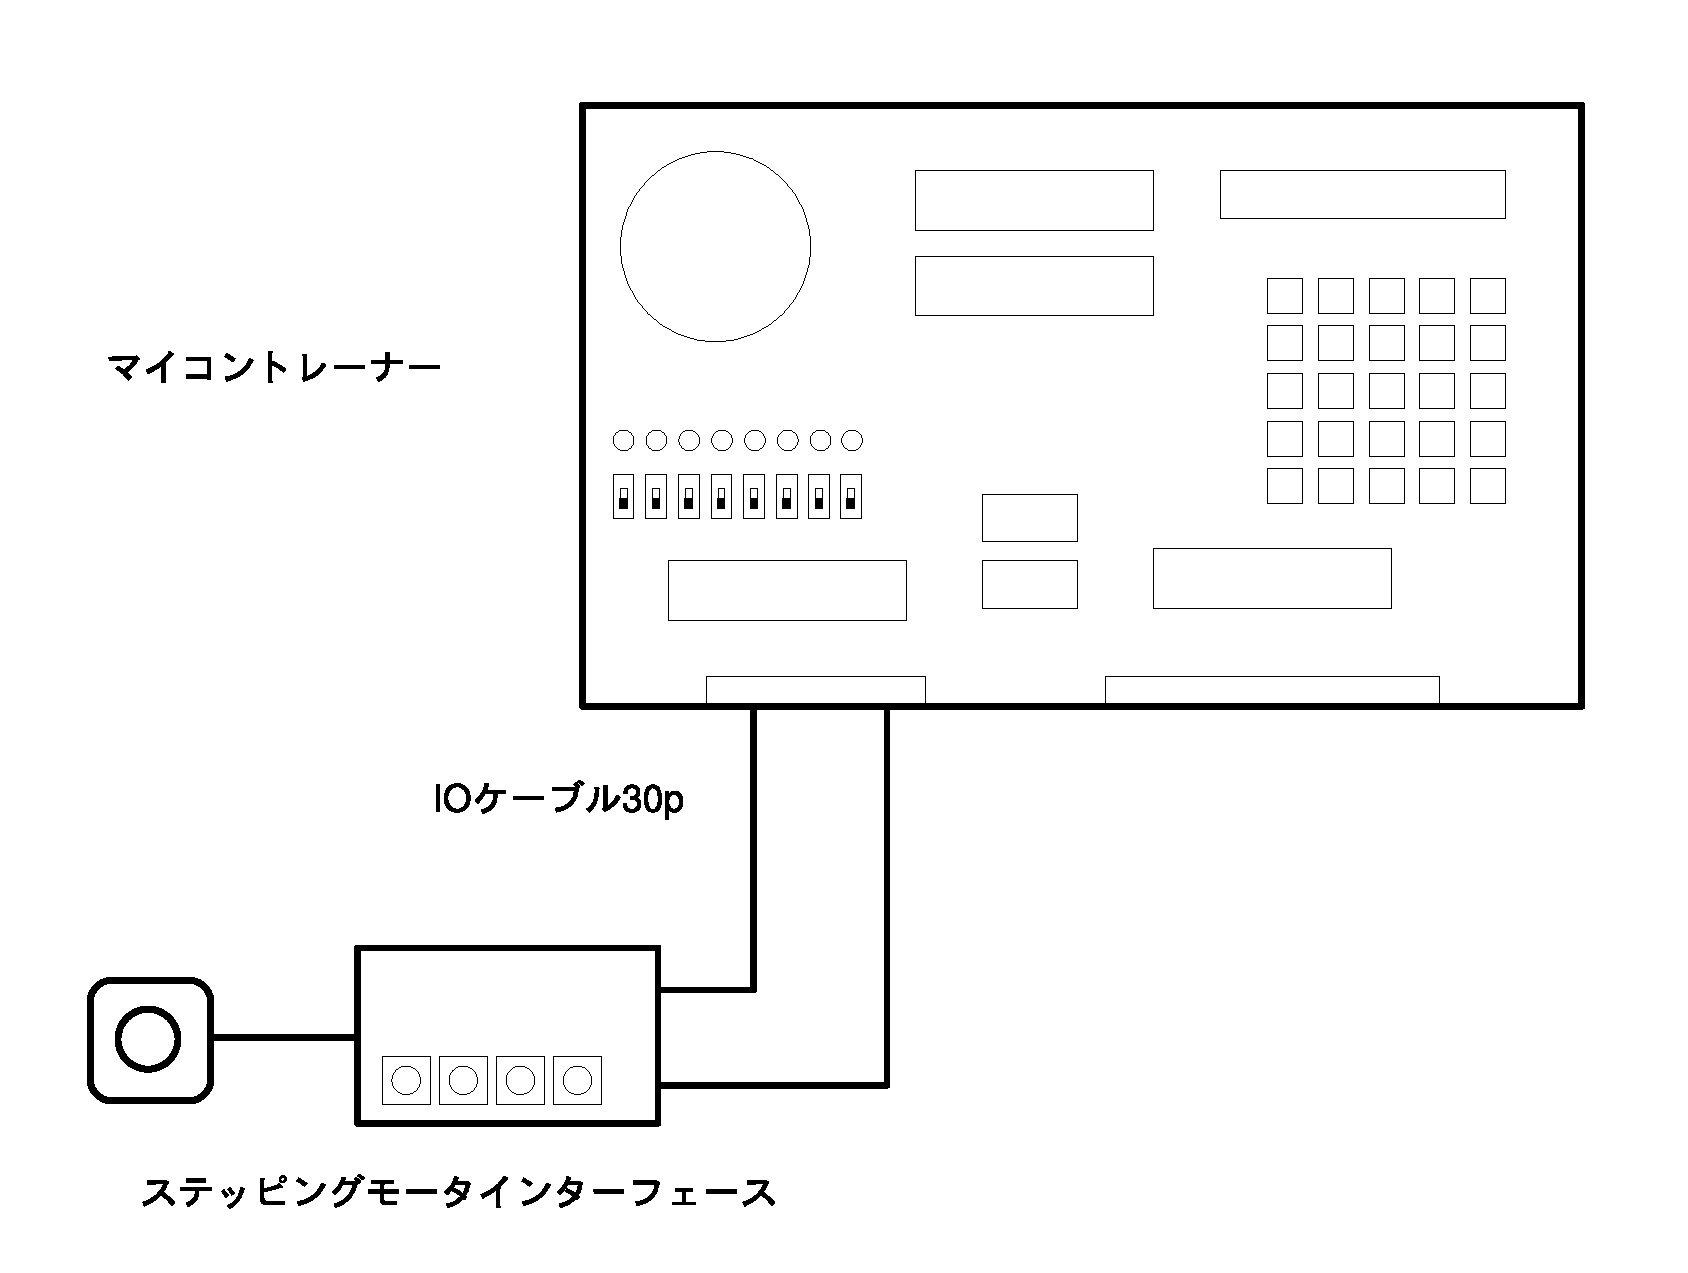
\includegraphics[width=0.8\linewidth]{img/connection-motor.eps}
\caption{マイコントレーナMT-Zとステッピングモータの接続図}
\label{fig:connection-motor}
\end{center}
\end{figure}

\section{実験}
ステッピングモータを回転させます。ステッピングモータは, 流すパルス電流のパターン(ドライブパターン)を変える
ことで, 性質の異なった回転をさせることができます。今回は, 1相励磁回
転(\tabref{tab:1sou}), 2相励磁回転(\tabref{tab:2sou}), 1-2相励磁回転(\tabref{tab:12sou})の3種類のドライブパターンを行います。


\begin{description}
\item[課題1] \tabref{tab:1sou}は1相励磁回転のドライブパターンである。1相励磁回転をさせなさい(\tabref{tab:q2-1})。


\begin{table}
\begin{center}
\caption{1相励磁回転ドライブパターン}
\label{tab:1sou}
\begin{tabular}{|c|c|c|c|c|}
\hline
ステップ&PB0& PB1&  PB2&  PB3\\ \hline
       0&  1&   0&    0&    0\\ \hline
       1&  0&   1&    0&    0\\ \hline
       2&  0&   0&    1&    0\\ \hline
       3&  0&   0&    0&    1\\
\hline
\end{tabular}
\end{center}
\end{table}



\begin{table}
\begin{center}
\caption{課題1のプログラム}
\label{tab:q2-1}
\footnotesize
\begin{tabular}{|c|l|ll|l|}
\hline
アドレス& \multicolumn{1}{|c|}{機械語}&\multicolumn{1}{|c}{ラベル}&\multicolumn{1}{c|}{ニーモニック}&\multicolumn{1}{|c|}{コメント}\\
\hline
   0005 &            &   &PB EQU 05H& ポートBアドレス\\
   0007 &            &   &CTL EQU 07H& コントロールポートアドレス\\
   0091 &            &   &CLWD EQU 90H& コントロールワード\\
        &            &   &&\\
   8400 &            &   &    ORG 8400H&\\
   8400 &  \underline{~~~~} \underline{~~~~}     &   STPMTR:& LD A , CLWD& コン
                    トロールワードをAレジスタに転送\\
   8402 &  \underline{~~~~} \underline{~~~~}      &   &    OUT (CTL) , A & コン
                    トロールポートにAレジスタの値を出力\\
   8404 &  \underline{~~~~} \underline{~~~~}       &   LOOP:& LD A , 01H& 01Hを
                    Aレジスタに転送\\
   8406 &  \underline{~~~~} \underline{~~~~}      &   &   OUT (PB) , A   & Aレジ
                    スタの値をポートBに出力\\
   8408 &  \underline{~~~~} \underline{~~~~}  \underline{~~~~}   &   &   CALL
                TIMER& タイマを呼び出す\\
   840B &  \underline{~~~~} \underline{~~~~}      &   &   LD A , 02H& 02HをAレジ
                    スタに転送\\
   840D &  \underline{~~~~} \underline{~~~~}     &   &   OUT (PB) , A   & Aレジ
                    スタの値をポートBに出力\\
   840F &  \underline{~~~~} \underline{~~~~} \underline{~~~~}  &   &   CALL
                TIMER& タイマおよび出す\\
   8412 &  \underline{~~~~} \underline{~~~~}     &   &   LD A , 04H& 04HをAレジ
                    スタに転送\\
   8414 &  \underline{~~~~} \underline{~~~~}      &   &   OUT (PB) , A   & Aレジ
                    スタの値をポートBに出力\\
   8416 &  \underline{~~~~} \underline{~~~~} \underline{~~~~}   &   &   CALL
                TIMER& タイマを呼び出す\\
   8419 &  \underline{~~~~} \underline{~~~~}      &   &   LD A , 08H& 08HをAレジ
                    スタに転送\\
   841B &  \underline{~~~~} \underline{~~~~}     &   &   OUT (PB) , A   & Aレジ
                    スタの値をポートBに出力\\
   841D &  \underline{~~~~} \underline{~~~~} \underline{~~~~}   &   &   CALL
                TIMER& タイマを呼び出す\\
   8420 &  \underline{~~~~} \underline{~~~~} \underline{~~~~}   &   &   JP LOOP& ループにジャン
                    プ\\
        &            &   &&\\
   8440 &            &    &    ORG 8440H&\\
   8440 &  21 00 40   &    TIMER:& LD
                HL , 4000H& 値4000HをHLレジスタに転送\\
   8443 &  5F        &    &    LD E, A&Aレジスタの値をEレジスタに
                    転送\\
   8444 &  2B        &    TLOOP:& DEC HL&HLレジスタの値から1を引く\\
   8445 &  7C        &    &    LD A, H&Hレジスタの値をAレジスタに
                    転送\\
   8446 &  B5        &    &    OR L& Aの値とLの値の論理和をとる\\
   8447 &  20 FB       &    &    JR NZ , TLOOP& フ
                    ラグレジスタがNZならばTLOOPにジャンプ\\
   8449 &  7B        &    &    LD A, E& Eレジスタの値をAレジスタに
                    転送\\
   844A &  C9        &    &    RET&ルーティンの終了\\
   844B &            &    &    END&\\
\hline
\end{tabular}
\end{center}
\end{table}



\item[課題2] \tabref{tab:2sou}は2相励磁回転のドライブパターンである。課題1のプ
           ログラムを参考に, ステッピングモータを2相励磁回転させよ。

\begin{table}
\begin{center}
\caption{2相励磁回転ドライブパターン}
\footnotesize
\begin{tabular}{|c|c|c|c|c|}
\hline
ステップ&PB0& PB1&  PB2&  PB3\\ \hline
       0&  1&   1&    0&    0\\ \hline
       1&  0&   1&    1&    0\\ \hline
       2&  0&   0&    1&    1\\ \hline
       3&  1&   0&    0&    1\\
\hline
\end{tabular}
\end{center}
\label{tab:2sou}
\end{table}


\item[課題3] \tabref{tab:12sou}は1--2相励磁回転のドライブパターンである。課題1のプ
           ログラムを参考に, ステッピングモータを1--2相励磁回転させよ。

\begin{table}
\begin{center}
\caption{1--2相励磁回転ドライブパターン}
\label{tab:12sou}
\footnotesize
\begin{tabular}{|c|c|c|c|c|}
\hline
ステップ&PB0& PB1&  PB2&  PB3\\ \hline
       0&  1&   0&    0&    0\\ \hline
       1&  1&   1&    0&    0\\ \hline
       2&  0&   1&    0&    0\\ \hline
       3&  0&   1&    1&    0\\ \hline
       4&  0&   0&    1&    0\\ \hline
       5&  0&   0&    1&    1\\ \hline
       6&  0&   0&    0&    1\\ \hline
       7&  1&   0&    0&    1\\
\hline
\end{tabular}
\end{center}
\end{table}

\end{description}

\section{スイッチ操作の復習}

ここでは, スイッチ操作の復習を行います。スイッチは, MT-Z上の8255AのポートAにつな
がっています。ポートAを入力モードにすることでスイッチからの信号を入力することが
できるようになります。よって, ここでもコントロールワードは90Hを用いることになり
ます。


\begin{description}
\item[課題4] スイッチの状態を読み込んで, それをLEDに出力するプログラムを作りなさ
           い(\tabref{tab:q2-4})。


\begin{itemize}
\item ポートの信号を入力する場合は``IN''を使います。
\end{itemize}

\begin{table}
\begin{center}
\caption{課題4のプログラム}
\label{tab:q2-4}
\footnotesize
\begin{tabular}{|c|l|ll|l|}
\hline
アドレス& \multicolumn{1}{|c|}{機械語}&\multicolumn{1}{|c}{ラベル}&\multicolumn{1}{c|}{ニーモニック}&\multicolumn{1}{|c|}{コメント}\\
\hline
   0004 &           & & PA EQU 04H& ポートAアドレス\\
   0005 &           & & PB EQU 05H& ポートBアドレス\\
   0007 &           & & CTL EQU 07H& コントロールポートアドレス\\
   0090 &           & & CLWD EQU 90H& コントロールワード\\
        &           & & &\\
   8400 &           & &     ORG 8400H&\\
   8400 & \underline{~~~~} \underline{~~~~}      & &     LD A, CLWD& コントロー
                    ルワード\\
   8402 & \underline{~~~~} \underline{~~~~}      & &     OUT (CTL), A& コントロー
                    ルポートにAレジスタの値を出力\\
   8404 & \underline{~~~~} \underline{~~~~}      &  LOOP:& IN A, (PA)& ポートAか
                    らAレジスタに入力\\
   8406 & \underline{~~~~} \underline{~~~~}     & &     OUT (PB), A& Aレジスタの
                    値をポートBに出力\\
   8408 & \underline{~~~~} \underline{~~~~} \underline{~~~~}   & &     JP LOOP&
                    LOOPにジャンプ\\
   840B &           & &     END&\\
\hline
\end{tabular}
\end{center}
\end{table}


\item[課題5] \figref{fig:flow4}を参考に, スイッチの右端がONの場合LEDの点灯を左にシフトさせ, OFFの場合停止
           させるプログラムを作りなさい。


\begin{figure}[htbp]
\begin{center}
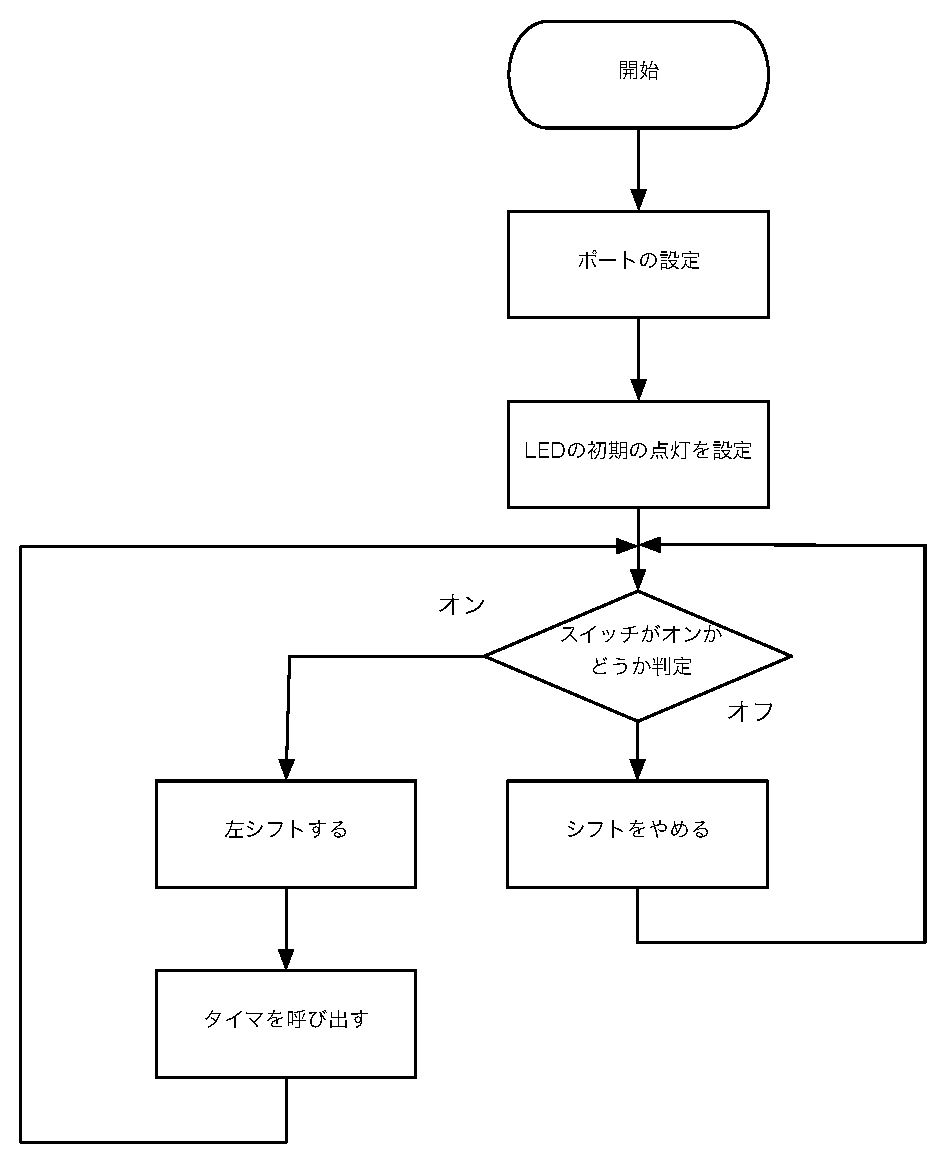
\includegraphics[width=0.8\linewidth]{img/flow4.eps}
\caption{課題5の処理の流れ}
\label{fig:flow4}
\end{center}
\end{figure}


\item[課題6] 2つの4桁の2進の数値を入力し, それを加算し結果をLEDで表示するプログ
           ラムを作りなさい。数値を入力する場合は, スイッチの右4つ, 左4つそれぞ
           れの状態を2つの4桁の数としなさい。

\end{description}

\newpage

\section{考察課題}

\begin{description}

\item[考察課題1] タイマサブルーティンはなぜ必要か答えなさい。

\item[考察課題2] 今回は3種類のドライブの仕方を行った。各ドライブパターンの特徴をしらべて報
      告しなさい。

\item[考察課題3] 課題1のプログラムをどのように変えると回転速度や回転方向が変わるか考えなさ
      い。
\end{description}